\subsection{Data Retrieval - Justin} \label{sec:data-retrieve}


\subsubsection{Scenario}
Bob in Dallas has heard people talk about the research Alice from Subsection~\ref{sec:data-insert} has been doing on the Hydra instance on FABRIC. So much so that Bob wants to see for himself what the data looks like. Of course, Bob (being a new user of the Hydra instance) has no idea where the data replicas are located. The replicas could not be on Dallas, the Hydra node he is most close to. Therefore, Bob needs a way to fetch Alice's data regardless of where the data is located within Hydra. To satisfy this scenario, the following interactions are conducted.


\subsubsection{User-to-Node Interaction}
The process of how a user fetches a file from Hydra can be described as a series of interests and data packets with the only difference being the segment number component. An important note is that any Hydra node can handle a user's fetch requests regardless of whether the contacted node has the file or not.

The user starts out by sending an interest who's name follows the form /<hydra-prefix>/fetch/<file-name>/<segment-no> with the filename being the name found within Hydra and the segment number being 0. The user will automatically assume the file spans multiple packets and always add the segment component to its interest. If the file only spans 1 packet, the user will find that out via the final block id within the first data packet. While fetching any a file starts the same, it does not end the same: there are 3 situations that can occur after expressing that interest.

The user's interest for file (F) can be fulfilled from the following:
\begin{enumerate}
    \item NACK: File (F) does not exist on Hydra.
    \item BLOB: File (F) exists on the contacted node, data is returned.
    \item ForwardingHint: File (F) exists in Hydra, but not on the contacted node. This acts as a redirect.
\end{enumerate}

To minimize traffic and be more precise with data retrieval, the user can first send an interest and see how the interest will be fulfilled which can tell the user how to proceed. After finding out the correct fetch path either by getting data or by a redirect, a user can concurrently send interests to get the rest of the file. If a NACK is received when sending the first interest, the user knows that the file is not within Hydra and to stop further interaction.

\subsubsection{Module Interaction}
\begin{figure}[!ht]
    \centering
    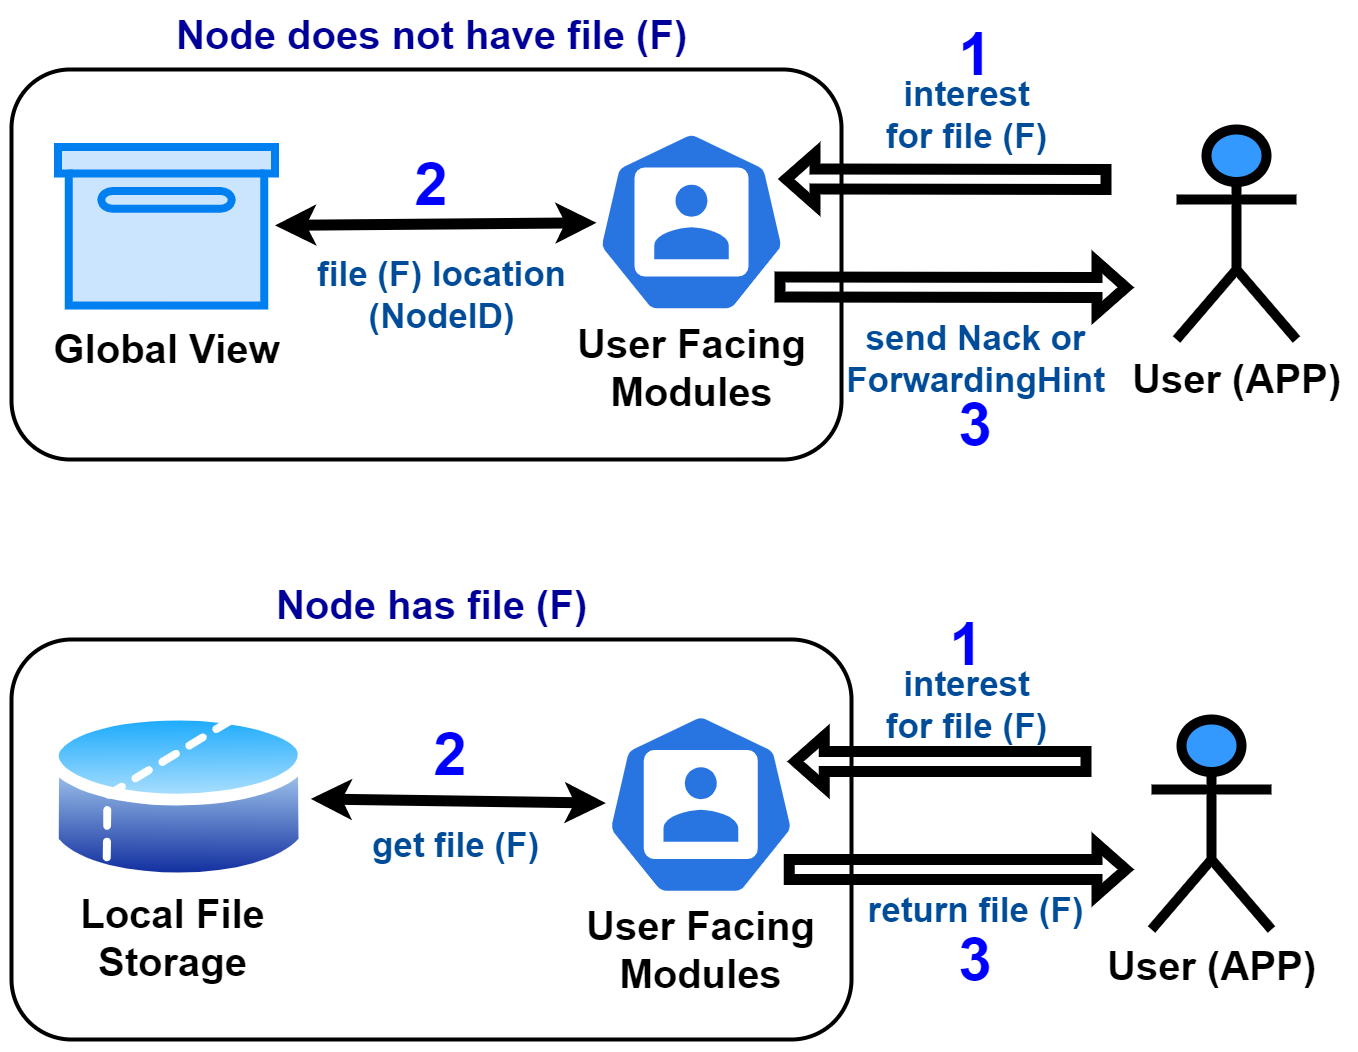
\includegraphics[width=\columnwidth]{visuals/fetch-sys.png}
    \caption{Module Interaction to Fulfill a User's Retrieval Requests}
    \label{fig:fetch-sys}
\end{figure}

Figure~\ref{fig:fetch-sys} shows two different situations. The Global View is used to indicate where the requested file is. After finding this information, the Hydra node responds to the user in the already-list 3 ways. In the case that the contacted node has the file, the local file storage is used to provide the file data. If a ForwardingHint is required, the node selects a random Hydra node that has the file and provides a unicast name (using the selected node's name) following the format /<node-name>/<hydra-prefix>/fetch/<file-name> for the user to use to fetch the file. Please note that this is the same format that a node uses to fetch a file from another node.